\documentclass[journal,10pt,twocolumn]{article}
\usepackage[margin=0.5in]{geometry}
\usepackage[cmex10]{amsmath}
\usepackage{amsmath}
\usepackage{array}
\usepackage{booktabs}
% The preceding line is only needed to identify funding in the first footnote. If that is unneeded, please comment it out.
\usepackage{cite}
\usepackage{amsmath,amssymb,amsfonts}
\usepackage{graphicx}
\usepackage{textcomp}
\usepackage{xcolor}
\graphicspath{{./figs/}}{}
\usepackage{amsmath,amssymb,amsfonts,amsthm}
\usepackage{gensymb}
\newcommand{\myvec}[1]{\ensuremath{\begin{pmatrix}#1\end{pmatrix}}}
\let\vec\mathbf
\title{
Matrix-Conic
}
\author{SHREYASH CHANDRA PUTTA}
\providecommand{\norm}[1]{\left\lVert#1\right\rVert}
\providecommand{\abs}[1]{\left\vert#1\right\vert}
\let\vec\mathbf
%\newcommand{\myvec}[1]{\ensuremath{\begin{pmatrix}#1\end{pmatrix}}}
\newcommand{\mydet}[1]{\ensuremath{\begin{vmatrix}#1\end{vmatrix}}}
\providecommand{\brak}[1]{\ensuremath{\left(#1\right)}}
\providecommand{\brak}[1]{\ensuremath{\left(#1\right)}}
\providecommand{\lbrak}[1]{\ensuremath{\left(#1\right.}}
\providecommand{\rbrak}[1]{\ensuremath{\left.#1\right)}}
\providecommand{\sbrak}[1]{\ensuremath{{}\left[#1\right]}}


\begin{document}
\maketitle
\tableofcontents
\bigskip
\section{Problem Statement}
To find the locus of mid point of $\vec{P\:Q}$ where $\vec{P}$ is (1,0) and $\vec{Q}$ is a point on the locus $y^{2} = 8x$ .

\section{Solution}
Let $\vec{X}$ be any point on the Locus formed by the midpoint joining the point $\vec{P}$ and any point on the given locus say, point $\vec{Q}$  \\

Where, 
  ${\vec{P}}$=$\myvec{
  1\\
  0}$
  ,${\vec{Q}}$=$\myvec{
  x'\\
  y'}$
 and ${\vec{X}}$=$\myvec{
  x\\
  y}$


The given equation of parabola $y^2 = 8x$ can be written in the general quadratic form as
\begin{align}
    \vec{x}^{\top}\vec{V}\vec{x}+2\vec{u}^{\top}\vec{x}+f=0
    \label{eq-1}
    \end{align}
where
\begin{align}
	\label{eq:V_matrix}
	\vec{V} &= \myvec{0 & 0\\0 & 1},
	\\
	\label{eq:u_vector}
	\vec{u} &= \myvec{-4\\0},
	\\
	\label{eq:f_value}
	f &= 0
	%\\
\end{align}
\\
Substitute $\vec{Q}$ and data in ($\ref{eq-1}$).
\\
\begin{align}
    \vec{Q}^{\top}\vec{V}\vec{Q}+2\vec{u}^{\top}\vec{Q}=0
    \label{eq-5}
    \end{align}

By section formula
mid point of line joining $\vec{P}$ and $\vec{Q}$ as $\vec{X}$ is:
 
 \begin{equation}
	\vec{X}=\frac{\vec{Q}+\vec{P}}{2}
	 \label{eq-6}
\end{equation}
\\
 \begin{equation}
	\vec{Q}=2\vec{X}-\vec{P}
	 \label{eq-7}
\end{equation}
\\
%%%%%%%%%%%%%%%%%%%%%%%%%%%%%%%
From ($\ref{eq-5}$) and ($\ref{eq-7}$) We get 

\begin{multline}
    (2\vec{X}-\vec{P})^{\top}\vec{V}(2\vec{X}-\vec{P})+2\vec{u}^{\top}(2\vec{X}-\vec{P})=0
     \label{eq-8}
    \end{multline}

\begin{multline}
    \label{eq:conic_quad_form}
    (2\vec{X}^{\top}\vec{V}-\vec{P}^{\top}\vec{V})(2\vec{X}-\vec{P})+2\vec{u}^{\top}2\vec{X}-2\vec{u}^{\top}\vec{P}=0
    \end{multline}

\begin{multline}
    \label{eq:conic_quad_form}
    (2\vec{X}^{\top}\vec{V}2\vec{X}-2\vec{X}^{\top}\vec{V}\vec{P})+2\vec{u}^{\top}2\vec{X}-2\vec{u}^{\top}\vec{P}=0
    \end{multline}
 
\begin{multline}
    \label{eq:conic_quad_form}
    4\vec{X}^{\top}\vec{V}\vec{X}+4\vec{u}^{\top}\vec{X}-2\vec{X}^{\top}\vec{V}\vec{P}-2\vec{u}^{\top}\vec{P}=0
    \end{multline}
        
\begin{equation}
    \label{eq:conic_quad_form}
    4\vec{X}^{\top}\vec{V}\vec{X}+4\vec{u}^{\top}\vec{X}+8=0
    \end{equation}

\begin{equation}
    \label{eq:conic_quad_form}
    \vec{X}^{\top}\vec{V}\vec{X}+\vec{u}^{\top}\vec{X}+2=0
    \end{equation}
%%%%%%%%%%%%%%%%%%%%%%%%%%%%%%%%%%%%%%%%%%%%%%%%%%%%%%%%
\\
Therefore, required Locus equation of the mid point of given point $\vec{P}$ and $\vec{Q}$ is obtained as:
\begin{equation}
    \label{eq-13}
    \vec{X}^{\top}\vec{V}\vec{X}+2\vec{u'}^{\top}\vec{X}+f'=0
    \end{equation}
%%%%%%%%%%%%%%%%%%%%%%%%%%%%%%%
where
\begin{align}
	\label{eq:V_matrix}
	\vec{V} &= \myvec{0 & 0\\0 & 1},
	\\
	\label{eq:u_vector}
	\vec{u'} &= \myvec{-2\\0},
	\\
	\label{eq:f_value}
	f' &= 2
	%\\
\end{align}
%%%%%%%%%%%%%%%%%%%%%%%%%%%%%%%%%%%%%%%%%%%%%%%%%
 \subsection{verification}

\textbf{Comparing }
generate point on the obtained locus as $\vec{X}$\\
then,\\ The intersection of given ($\ref{eq-1}$) with a line along $\vec{P}$ and $\vec{X}$. 
 \\And find If ($\ref{eq-6}$) is satisfied or not 

the point of intersection of the line with the conic section is considered as $\vec{Q}$
\\

From the above considerations below vectors are taken
\begin{align}
\vec{q} = \vec{X} ,\: \vec{m}=(\vec{X-P})
\end{align}


The points of intersection of the line, \\ 
\begin{align}
L: \quad \vec{x} = \vec{q} + \mu \vec{m} \quad \mu \in \mathbb{R}
\end{align}
with the conic section, \\ 
\begin{align}
	\vec{x}^{\top}\vec{V}\vec{x} + 2\vec{u}^{\top} \vec{x} + f = 0
\end{align}
are given by \\
\begin{align}
\vec{x}_i = \vec{q} + \mu_i \vec{m}
\label{eq-21}
\end{align}
%%%%%%%%%%%%%%%%%%%%%%%%%
where
{\tiny
\begin{multline}
\mu_i = \frac{1}
{
\vec{m}^T\vec{V}\vec{m}
}
\lbrak{-\vec{m}^T\brak{\vec{V}\vec{q}+\vec{u}}}
\\
\pm
\rbrak{\sqrt{
\sbrak{
\vec{m}^T\brak{\vec{V}\vec{q}+\vec{u}}
}^2
-
\brak
{
\vec{q}^T\vec{V}\vec{q} + 2\vec{u}^T\vec{q} +f
}
\brak{\vec{m}^T\vec{V}\vec{m}}
}
}
\label{eq-22}
\end{multline}
}

%%%%%%%%%%%%%%%%%%
\raggedright On substituting $\vec{V},\vec{u},\vec{q} ,\vec{m}$ in the above
equation,
we get the values of $\mu$. By substituting the values of $\mu$ in
($\ref{eq-21}$), \\we get the points of intersection of line with the given
curve. \\
\centering $i.e., \vec{x1},\vec{x2}$\\  we take only one of the suitable point in consideration to verify (\ref{eq-6})
in this way obtained locus is verified

\raggedright \section{Software}
Download the following code using,
\begin{table}[h]
    \centering
    \begin{tabular}{|c|}
    \hline \\
         svn co https://github.com/chanduputta/\\FWC-Module1Assignments/blob/\\main/conic/code/conic.py \\
         \\
\hline
    \end{tabular}
\end{table}
\\
and execute the code by using command
\begin{center}
\textbf{cmd1:}Python3  conic.py\\
\textbf{cmd2:}Input y-coordinate to generate point on locus\\
\textbf{Observe:} the obtained locus is verified or not\\
\end{center}

\raggedright \section{Plotting}
{\begin{table}[h]
    \centering
    \begin{tabular}{|c|c|c|}
       \hline
       \textbf{Symbol}&\textbf{Value}&\textbf{Description}  \\
       \hline
	    $\vec{P}$ & $\myvec{
		    1\\
		    0}$
	    & given point\\
        \hline
	    $\vec{Q}$ & $\myvec{x'\\y'}$
 &  point on given locus \\
        \hline
	    $\vec{X}$ & $\myvec{x\\y}$
 & mid point of $\vec{PQ}$  \\
       \hline
    \end{tabular}
    \caption{Parameters}
    \label{tab:my_label}
\end{table}

\begin{figure}[h]
    \centering
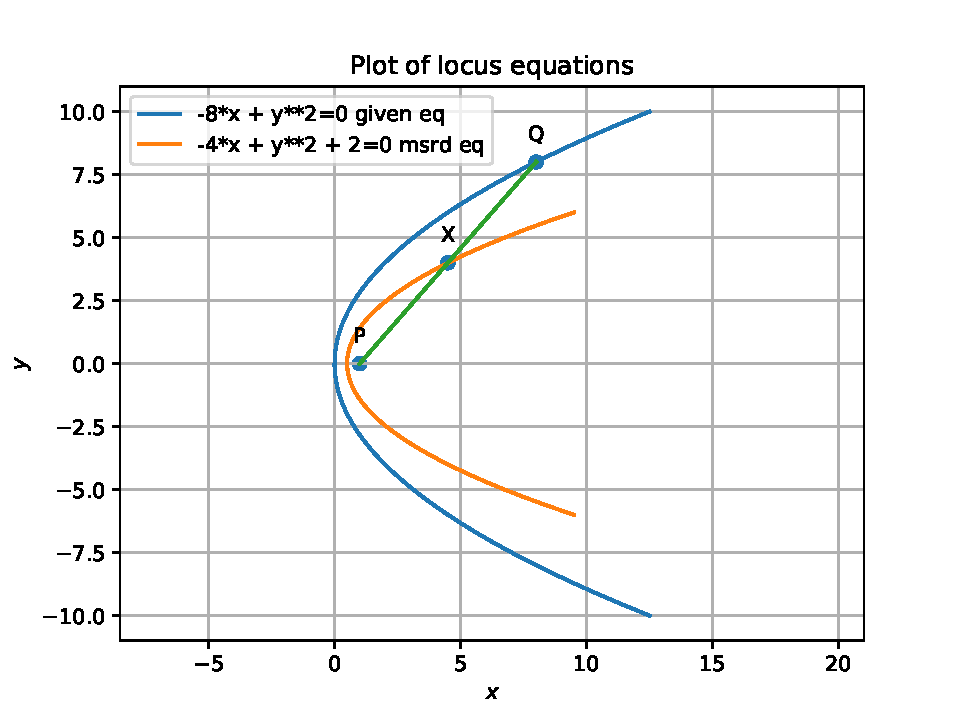
\includegraphics[width=\columnwidth]{fig/conicfig.pdf}
    \caption{Found the locus equation }
    \label{fig:my_label}
\end{figure}
\vspace{2cm}
}
\raggedright \section{Conclusion}
\begin{center}
We found the locus of mid point of $\vec{P\:Q}$ where $\vec{P}$ is (1,0) and $\vec{Q}$ is a point on the locus $\vec{y^{2} = 8x}$ as $\vec{y^{2} = 4x - 2}$ and Verified.
\end{center}
\end{document}
